\documentclass{article}

\usepackage{graphicx}
\usepackage{tikz}
\usepackage{tikzsymbols}
\usetikzlibrary{calc,patterns,shapes.geometric}
\pagestyle{empty}
\usepackage[margin=0pt]{geometry}
\geometry{papersize={14in,12in}}

\def\centerarc[#1](#2)(#3:#4:#5){\draw[#1] ($(#2)+({#5*cos(#3)},{#5*sin(#3)})$) arc (#3:#4:#5);}

\begin{document}
	\begin{figure}
		\centering
		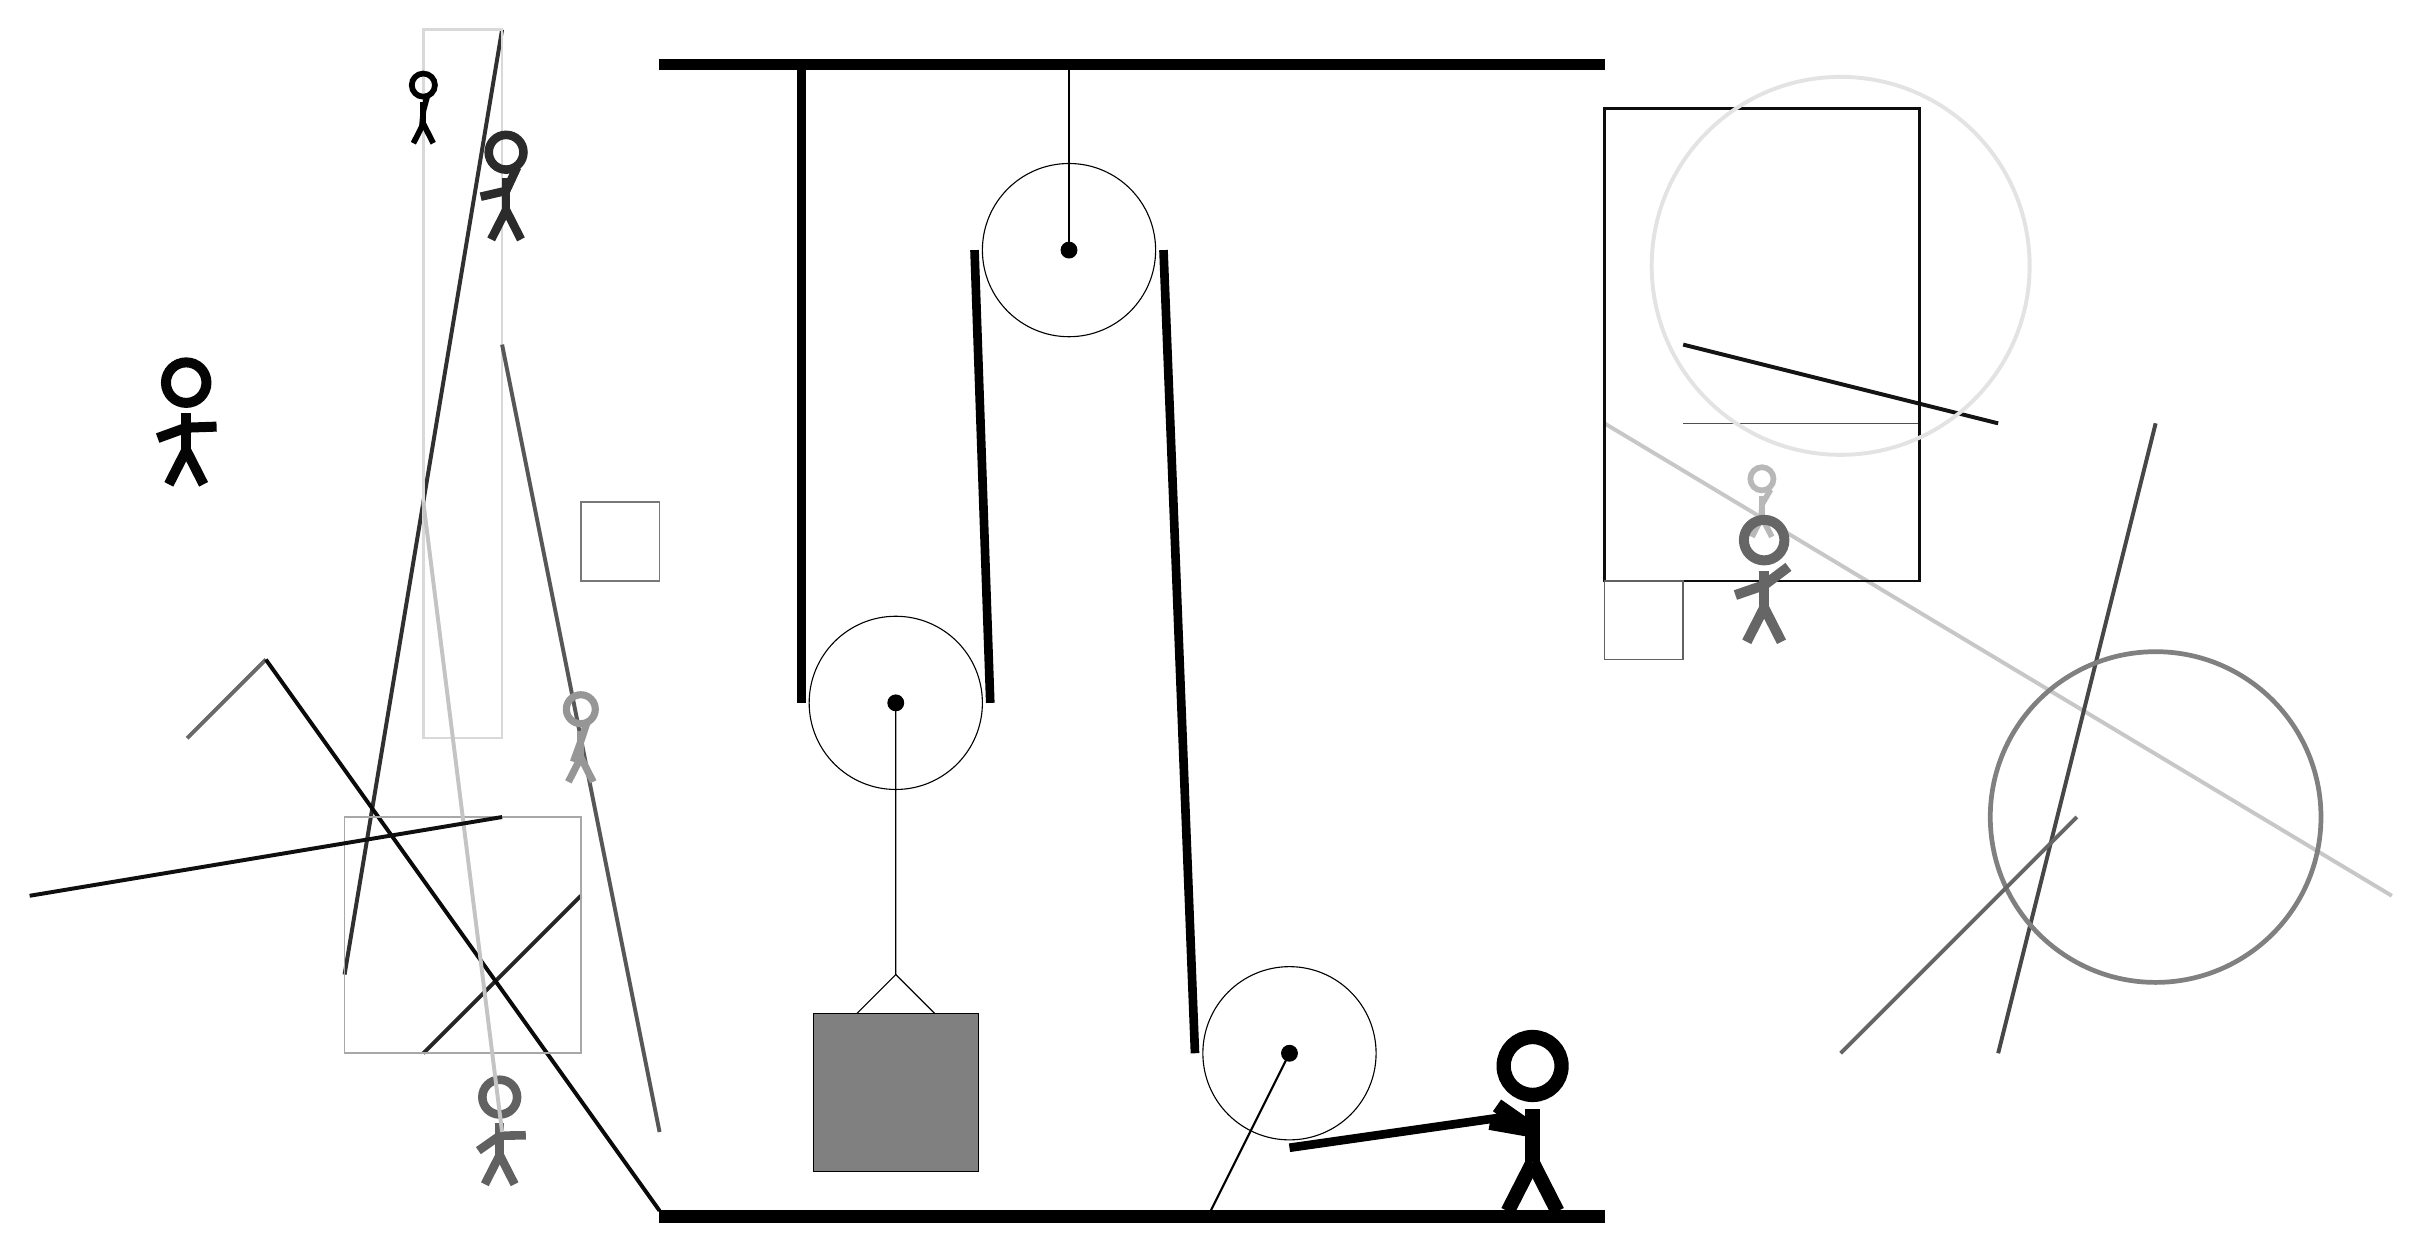
\begin{tikzpicture}
			%%%%% START %%%%%
			
			\draw[fill=black] (-2, 11.5) rectangle (10, 11.625);
			
			\draw (3.2, 9.2) circle (1.1);
			\draw[fill=black] (3.2, 9.2) circle (0.1);
			\draw[thick] (3.2, 9.2) -- (3.2, 11.5);
			
			\draw (6, -1) circle (1.1);
			\draw[fill=black] (6, -1) circle (0.1);
			\draw[thick] (6, -1) -- (5, -3);
			
			\draw (1, 3.45) circle (1.1);
			\draw[fill=black] (1, 3.45) circle (0.1);
			
			\draw[line width=0.5mm, color=black!22](10, 7) -- (20, 1);
			
			\draw[line width=0.5mm, color=black!81](-4, 12) -- (-6, 0);
			\draw[line width=0.3mm, color=black!15] (-4, 3) rectangle (-5, 12);
			\node[line width=0.2mm, color=black!62] at (-4, -2) {\Strichmaxerl[6][35][1]};
			\draw[line width=0.5mm, color=black!59](-7, 4) -- (-8, 3);
			
			\node[line width=0.5mm, color=black!83] at (-4, 10) {\Strichmaxerl[6][13][65]};
			\draw[line width=0.5mm, color=black!85](-5, -1) -- (-3, 1);
			
			\draw[line width=0.5mm, color=black!72](15, -1) -- (17, 7);
			\draw[line width=0.5mm, color=black!96](-2, -3) -- (-7, 4);
			\draw[line width=0.5mm, color=black!66](-2, -2) -- (-4, 8);
			\node[line width=0.3mm, color=black!28] at (12, 6) {\Strichmaxerl[4][87][60]};
			
			\node[line width=0.7mm, color=black!100] at (-5, 11) {\Strichmaxerl[4][85][75]};
			\draw[line width=0.2mm, color=black!34] (-3, -1) rectangle (-6, 2);
			\draw[line width=0.5mm, color=black!92](15, 7) -- (11, 8);
			\draw[line width=0.5mm, color=black!23](-4, -2) -- (-5, 6);
			\draw[line width=0.7mm, color=black!75] (11, 1) rectangle (11, 1);
			\draw [line width=0.6mm, color=black!50](17, 2) circle (2.1);
			
			\draw[line width=0.5mm, color=black!94](-4, 2) -- (-10, 1);
			\draw[line width=0.2mm, color=black!53] (-2, 6) rectangle (-3, 5);
			
			\node[line width=0.2mm, color=black!98] at (-8, 7) {\Strichmaxerl[7][20][2]};
			\draw[line width=0.2mm, color=black!69] (11, 7) rectangle (14, 7);
			
			\draw[line width=0.3mm, color=black!95] (10, 11) rectangle (14, 5);
			\draw [line width=0.5mm, color=black!11](13, 9) circle (2.4);
			\node[line width=0.7mm, color=black!41] at (-3, 3) {\Strichmaxerl[5][70][72]};
			\node[line width=0.5mm, color=black!60] at (12, 5) {\Strichmaxerl[7][19][37]};
			
			\draw[line width=0.2mm, color=black!62] (11, 4) rectangle (10, 5);
			\draw[line width=0.5mm, color=black!60](13, -1) -- (16, 2);
			
			\draw (1, 3.45) -- (1, 0.0) -- (0.5, -0.5);
			\draw (1, 0.0) -- (1.5, -0.5);
			\draw[fill=black!50] (-0.05, -0.5) rectangle (2.05, -2.5);
			
			\draw[line width=1.1mm] (-0.2, 11.5) -- (-0.2, 3.45);
			\centerarc[line width=1.1mm](1, 3.45)(180:360:1.2000000000000002);
			\draw[line width=1.1mm](2.2, 3.45) -- (2.0, 9.2);
			\centerarc[line width=1.1mm](3.2, 9.2)(0:180:1.2000000000000002);
			\draw[line width=1.1mm](4.4, 9.2) -- (4.8, -1);
			\centerarc[line width=1.1mm](6, -1)(180:270:1.2000000000000002);
			\draw[line width=1.1mm](6, -2.2) -- (8.8, -1.8);
			
			\node at (9, -1.9) {\Strichmaxerl[10][-35][170]};
			
			\draw[fill=black] (-2, -3) rectangle (10, -3.15);
			
			%%%%% END %%%%%
		\end{tikzpicture}
	\end{figure}	
\end{document}